\documentclass[11pt]{article}
\pdftrailerid{}
\usepackage[T1]{fontenc}
\usepackage{lmodern,microtype}
\usepackage[margin=1in]{geometry}
\usepackage{amsmath,amssymb,amsthm,mathtools}
\usepackage{tikz}
\usetikzlibrary{arrows.meta}
\usepackage[colorlinks=true,linkcolor=blue!50!black,citecolor=blue!50!black,urlcolor=blue!50!black]{hyperref}
\newtheorem{theorem}{Theorem}
\newtheorem{proposition}[theorem]{Proposition}
\newtheorem{lemma}[theorem]{Lemma}
\newtheorem{corollary}[theorem]{Corollary}
\newtheorem{remark}[theorem]{Remark}
\newcommand{\R}{\mathbb R}
\newcommand{\N}{\mathbb N}
\newcommand{\av}[2]{\frac{1}{|#1|}\int_{#1} #2}
\newcommand{\norm}[1]{\left\lVert#1\right\rVert}
\newcommand{\inner}[2]{\langle #1,#2\rangle}
\DeclareMathOperator{\diam}{diam}
\title{A doubling Hilbert subset with no finite-dimensional bi-Lipschitz embedding}
\author{OpenAI}
\hypersetup{pdftitle={A doubling Hilbert subset with no finite-dimensional bi-Lipschitz embedding},pdfauthor={OpenAI}}
\date{September 25, 2026}
\begin{document}
\maketitle
\begin{abstract}
Every infinite-dimensional real Banach space contains a compact doubling subset that admits no bi-Lipschitz embedding into any finite-dimensional real normed space. The doubling constant has a universal bound, independent of the ambient Banach space. This answers the Lang--Plaut problem negatively, even for compact subsets of Hilbert space.
\end{abstract}

\section{Introduction}
\label{sec:introduction}
A metric space $(X,d)$ is \emph{doubling with constant at most $\lambda$} if every ball in $X$ is covered by at most $\lambda$ balls of half its radius, with centers in $X$. A map $f:X\to\R^k$ is a \emph{bi-Lipschitz embedding with distortion at most $D$} if there is a scale $a>0$ such that
\[
 a\,d(x,y)\le\norm{f(x)-f(y)}\le Da\,d(x,y)
 \qquad(x,y\in X).
\]
Both the target dimension $k$ and the distortion $D$ are required to be finite.

Every subset of a finite-dimensional Euclidean space is doubling. Lang and Plaut asked whether every doubling subset of Hilbert space admits a bi-Lipschitz embedding into some finite-dimensional Euclidean space; see \cite[Question 2.4]{LP}, restated in \cite[Question 1]{NN}. Gupta, Krauthgamer, and Lee independently formulated the question in the context of algorithmic dimension reduction \cite[Section 6, Question 1]{GKL}. The hypothesis already supplies a Hilbert-space realization, so the issue is whether a bound on metric covering complexity permits a reduction to finitely many Euclidean coordinates while preserving all distances up to a fixed factor.

Assouad's theorem gives a positive result after changing the metric: every doubling metric space admits such an embedding for the distance $d^\alpha$, where $0<\alpha<1$ \cite{Assouad}. This operation is called \emph{snowflaking}. Naor and Neiman proved that, when $\alpha$ is close to $1$, the target dimension can be bounded in terms of the doubling constant alone, independently of $\alpha$ \cite[Theorem 1.2]{NN}. The distortion bound still depends on the snowflake exponent. For finite Hilbert subsets, Gottlieb and Krauthgamer obtained embeddings of snowflakes with distortion arbitrarily close to one, with dimension depending on the doubling constant, exponent, and permitted distortion \cite[Theorem 1.2]{GK}. The Lang--Plaut question concerns the original distance $d$, even when arbitrary finite dimension and distortion are allowed.

For exponents $p>2$, Lafforgue and Naor constructed doubling subsets of $L_p$ admitting no bi-Lipschitz embedding into any finite-dimensional Euclidean space \cite[Theorem 1.1]{LN}. Independently, Bartal, Gottlieb, and Neiman obtained dimension-reduction obstructions for doubling subsets of $\ell_p$ using thin Laakso configurations \cite{BGN}. Baudier, \'Swi\k{e}cicki, and Swift later gave an elementary proof of the corresponding fixed-set theorem for $\ell_q$, $q>2$ \cite[Theorem 1]{BSS}. These results concern ambient exponents strictly greater than two and do not settle the Hilbert case. Schioppa announced a negative answer in \cite{Schioppa}, but withdrew the preprint after reporting a possible issue with its duality argument.

We give a negative answer to this question.
\begin{theorem}\label{thm:main}
There is a fixed subset $S$ of real $\ell_2$, equipped with its induced Hilbert distance, whose doubling constant is at most $76800$ and which admits no bi-Lipschitz embedding into $\R^k$ for any positive integer $k$, at any finite distortion.
\end{theorem}
In particular, dimension and distortion bounds depending only on the doubling constant cannot hold for all doubling Hilbert subsets.

The same metric space has an isometric realization in $L_p([0,1];\R)$ for every $1\le p<\infty$, by a normalized Gaussian series; Section~\ref{sec:lp} gives this consequence and its relation to earlier $L_p$ obstructions. Section~\ref{sec:banach} constructs a compact obstruction in every infinite-dimensional real Banach space, including Hilbert space, with a universal doubling constant and with no bi-Lipschitz embedding into any finite-dimensional real normed space.

\subsection{The construction and proof strategy}
The proof couples a covering argument with a derivative obstruction. Differentiation has a substantial history as a method for ruling out Euclidean embeddings: Cheeger's framework gives such obstructions under doubling-measure and Poincar\'e-inequality hypotheses \cite[Section 14, Theorem 14.3]{Cheeger}. Laakso's nonembedding argument gives a related separation-versus-stretch principle: separated branches force an increase in stretch along a subsegment \cite[Section 4, Theorem 4.1]{Laakso}. Here the analytic step uses ordinary Euclidean differentiation of Lipschitz maps on open subsets of $\R^2$ and a quadratic variance identity. A lexicographic extremum treats the two derivative columns successively, and crossings turn their small variation into a packing obstruction. We describe the geometry first.

\paragraph{Sparse scales and common sheets.}
At each scale $r_j=1000^{-j}$, we color horizontal strips of width $r_j$ and vertical strips of width $W_jr_j$ periodically with $N_j$ colors. Here $N_j,W_j$ are positive integers, fixed in advance so that every pair occurs infinitely often. Choose unit vectors $e_{j,i}$, one for each level and color, mutually orthogonal and orthogonal to the base plane. For a base point $p\in\R^2$, color $i$ permits a displacement $r_je_{j,i}$ whenever $p$ is in a horizontal or a vertical strip of that color. Points of $S$ carry finitely many such displacements. Section~\ref{sec:construction} defines this set and proves the doubling bound: at any observation radius, the coarser coordinates are fixed, the finer coordinates have a small total diameter, and at most one intermediate level contributes labels to the cover.

Now suppose that an embedding $f$ exists, normalized to have lower Lipschitz constant one and upper constant $D$. Fixing a finite-support tuple of displacement coordinates and varying $p$ gives a map from an open part of the base plane to $\R^k$; we call this map a \emph{sheet}. If $F$ is one sheet and $F_i$ is obtained by adding a color-$i$ displacement at an unused level of size $r$, then
\[
 \norm{F_i(p)-F(p)}\le Dr
\]
wherever the added displacement is permitted. The horizontal and vertical restrictions belong to the same map $F_i$. Our objective is to find one horizontal line and one vertical line of each color along which the relative offset $(F_i-F)/r$ is nearly constant.

\paragraph{Two derivative extrema and two different error bounds.}
The derivative of each sheet has horizontal and vertical columns. Section~\ref{sec:extrema} takes the closure of all pairs of their squared norms, chooses the largest first coordinate $A$, and then chooses the largest second coordinate $B$ among pairs whose first coordinate is $A$. Near this extremal pair, a mean derivative close to a reference vector forces small mean-square variation. This elementary rigidity is the analytic input.

Fix the embedding parameters $k,D$, and then fix a color count $N$ larger than the number of points with pairwise distances greater than one that can fit in a radius-$D$ ball of $\R^k$. For each positive integer $n$, use a recurring level with $(N_j,W_j)=(N,n)$ inside a sufficiently small region of a nearly extremal sheet. Writing $r$ for its displacement scale, one period block contains one row and one column of each color and has width $Nnr$ and height $Nr$. In Section~\ref{sec:energy}, the first extremum gives horizontal derivative error whose mean square, multiplied by $n^2$, tends to zero. This factor compensates for the longer horizontal lines. The wide vertical strips first force the mean squared horizontal derivative norm of the vertically selected sheets toward $A$. The second extremum then gives vertical mean-square error tending to zero, with no growing factor required. Compactness suffices for this latter estimate; no quantitative modulus of the second extremum is needed.

\paragraph{Crossings turn small variation into a contradiction.}
Section~\ref{sec:crossings} selects one period block and a line of every color in each direction with the required small errors. Absolute continuity turns the derivative estimates into nearly constant relative offsets on those lines. At the crossing of a color-$i$ row and a color-$m$ column with $i\ne m$, both displacements are permitted, and the corresponding source points are separated by $\sqrt2\,r$. Transport to the selected same-color intersections therefore produces $N$ separated vectors in a radius-$D$ ball of $\R^k$. Euclidean volume comparison contradicts the choice of $N$. The fixed set is used throughout; only the sheets, local rectangles, and recurring level vary with $n$.

\subsection{Conventions}
Write $\N=\{1,2,\ldots\}$. In the proof of Theorem~\ref{thm:main}, all norms are Euclidean or Hilbert norms. For a Lipschitz map $F$ on an open subset of $\R^2$, write $F_x,F_y$ for its derivative columns, defined almost everywhere. For an integrable function $h$ on a set $E$ of positive finite area, write
\[
 \langle h\rangle_E=\frac{1}{|E|}\int_E h.
\]
The notation $\langle h\rangle$ omits $E$ when the averaging domain has been specified.

\section{The subset and its doubling bound}
\label{sec:construction}
We first construct the set independently of any target map. The rapid separation of the displacement scales will give a uniform covering bound even though the number of colors is unbounded.

Fix, once and for all, a sequence $(N_j,W_j)_{j\ge1}$ of pairs in $\N^2$ in which every pair occurs infinitely often. For example, concatenate the finite lists $\{1,\ldots,m\}^2$ for $m=1,2,\ldots$. Put $r_j=1000^{-j}$ and let
\[
 \mathcal H=\R^2\oplus\bigoplus_{j\ge1}\R^{N_j}
\]
be the Hilbert direct sum. This is isometric to real $\ell_2$. Let $e_{j,i}$, $1\le i\le N_j$, denote the coordinate vectors in its $j$th summand.

At level $j$, color the horizontal strips
\[
 \{(x,y):qr_j<y<(q+1)r_j\},\qquad q\in\mathbb Z,
\]
by the residue $i\in\{1,\ldots,N_j\}$ determined by $q\equiv i-1\pmod{N_j}$. Give the vertical strips
\[
 \{(x,y):qW_jr_j<x<(q+1)W_jr_j\}
\]
the same periodic coloring. Denote their unions of color $i$ by $H_{j,i}$ and $V_{j,i}$, respectively, and put
\[
 U_{j,i}=H_{j,i}\cup V_{j,i}.
\]
In particular, $U_{j,i}$ is open.

Define $S\subset\mathcal H$ to consist of the points
\begin{equation}\label{eq:set}
 (p,w),\qquad p\in\R^2,\quad w=(w_j)_{j\ge1},
\end{equation}
where $w$ has finite support and, independently at each level,
\[
 w_j=0\quad\text{or}\quad w_j=r_je_{j,i}\text{ for some }i\text{ with }p\in U_{j,i}.
\]
The zero choice is always allowed, including on strip boundaries. Neither $S$ nor its defining parameters will subsequently depend on a proposed embedding.

\begin{proposition}\label{prop:doubling}
The doubling constant of $S$ is at most $300\cdot16^2=76800$.
\end{proposition}
\begin{proof}
Fix a ball of radius $t>0$ centered at a point of $S$. Distinct choices of $w_j$ have distance at least $r_j$. Thus at every level with $r_j>t$, all points of the ball have the same coordinate as its center.

There is at most one intermediate level satisfying $t/64<r_j\le t$, since consecutive radii have ratio $1000$. The projection of the ball onto each base coordinate lies in an interval of length $2t$. Such an interval meets at most $\lfloor2t/r_j\rfloor+2\le129$ strips of width $r_j$, and the same upper bound applies to strips of width $W_jr_j\ge r_j$. Consequently, at the intermediate level there are fewer than $300$ available labels, including zero.

For any two points of the ball, the fine-coordinate distance is bounded by
\begin{equation}\label{eq:tail}
 \sum_{r_j\le t/64}\norm{w_j-w'_j}^2
 \le 2\sum_{r_j\le t/64}r_j^2
 \le\frac{2}{1-10^{-6}}\left(\frac{t}{64}\right)^2
 <\left(\frac{t}{32}\right)^2.
\end{equation}
Partition a base square of side $2t$ containing the projection into $16^2$ cells of side $t/8$, assigning their boundaries arbitrarily. Group the ball's points according to their cell and their intermediate coordinate, if one exists. In a group, the coarse and intermediate coordinates agree, the base diameter is at most $\sqrt2\,t/8$, and \eqref{eq:tail} bounds the fine coordinates. Each group therefore has diameter less than
\[
 t\sqrt{\frac{2}{64}+\frac{1}{1024}}=\frac{\sqrt{33}}{32}t<\frac t2.
\]
Choosing one point from each nonempty group as a center gives the required cover by balls in $S$.
\end{proof}

\section{Sheets and extremal derivatives}
\label{sec:extrema}
We now assume an embedding exists and extract one compact set of derivative data from all its sheets. Maximizing the two coordinates in order will constrain variation in the two directions separately.

Since $S$ contains the base plane with all displacement coordinates zero, it cannot embed into $\R^0$. Suppose, for a contradiction, that for some finite $k\ge1$ and $D\ge1$ there is a map $f:S\to\R^k$ satisfying
\begin{equation}\label{eq:bilip}
 \norm{z-z'}\le\norm{f(z)-f(z')}\le D\norm{z-z'}
 \qquad(z,z'\in S).
\end{equation}
For a fixed finite-support tuple $w$ of coordinate choices, let
\[
 \Omega_w=\{p:(p,w)\in S\}.
\]
If $w_j=r_je_{j,i_j}$ at its nonzero levels, then
\[
 \Omega_w=\bigcap_{j:w_j\ne0}U_{j,i_j}.
\]
This is a finite intersection of open sets; the empty intersection for the zero tuple is $\R^2$. Whenever the domain is nonempty, the map
\[
 F_w:\Omega_w\to\R^k,\qquad F_w(p)=f(p,w),
\]
is called a \emph{sheet}. It is $D$-Lipschitz, since the corresponding source points differ only in their base coordinates. This holds even when its domain is disconnected.

Rademacher's theorem gives differentiability almost everywhere on each sheet domain \cite[Theorem 3.1]{Heinonen}. Its derivative columns have norm at most $D$. By Lebesgue differentiation, almost every point $p$ is also a Lebesgue point of these columns; see \cite[Theorem 32 and Exercise 33]{Tao}. At such a point, with $u=F_x(p)$ and $v=F_y(p)$, the mean-square error satisfies
\begin{equation}\label{eq:good}
 \lim_{l\downarrow0}\left\langle\norm{F_x-u}^2+\norm{F_y-v}^2\right\rangle_{Q(p,l)}=0,
\end{equation}
where $Q(p,l)$ is the centered square of side $l$. Indeed, boundedness upgrades the Lebesgue mean-norm conclusion to mean-square convergence, and squares may replace balls by area comparison. Call these differentiability and Lebesgue points \emph{good}; they form a set of full measure in each sheet domain.

Let $K$ be the closure in $[0,D^2]^2$ of all pairs
\[
 (\norm{F_x(p)}^2,\norm{F_y(p)}^2)
\]
from all sheets and their good points. It is nonempty and compact. Define
\begin{equation}\label{eq:AB}
 A=\max\{s:(s,t)\in K\},\qquad
 B=\max\{t:(A,t)\in K\}.
\end{equation}
Thus $(A,B)\in K$. This single compact set and these two numbers remain fixed throughout the argument. The next lemma explains the benefit of maximizing the coordinates in this order: if the mean deficit from $A$ tends to zero, then the mean second coordinate cannot exceed $B$ in the limit.

\begin{lemma}[Near the lexicographic maximum]\label{lem:compact}
Let $D>0$, let $K\subseteq[0,D^2]^2$ be nonempty and compact, and define
$A=\max\{s:(s,t)\in K\}$ and $B=\max\{t:(A,t)\in K\}$.
For every $\varepsilon>0$ there is $\delta>0$ such that
\[
 (s,t)\in K,\quad s>A-\delta\quad\Longrightarrow\quad t\le B+\varepsilon.
\]
Consequently, if measurable pairs $(s_n,t_n)$ take values in $K$ on probability spaces and $\mathbb E(A-s_n)\to0$, then
$\limsup_n\mathbb E t_n\le B$.
\end{lemma}
\begin{proof}
Failure of the first assertion would give a sequence in $K$ with first coordinate tending to $A$ and second coordinate greater than $B+\varepsilon$. A convergent subsequence would contradict the definition of $B$. For the second assertion, Markov's inequality gives
\[
 \mathbb P\{A-s_n\ge\delta\}\le\frac{\mathbb E(A-s_n)}{\delta},
 \qquad
 \mathbb E t_n\le B+\varepsilon+
 D^2\frac{\mathbb E(A-s_n)}{\delta}.
\]
First let $n\to\infty$, and then $\varepsilon\downarrow0$.
\end{proof}

The lemma supplies an upper bound on a mean squared norm. To turn that bound into small variation around a reference vector, we will also control the mean vector and use the elementary identity
\begin{equation}\label{eq:variance}
 \left\langle\norm{G-a}^2\right\rangle
 =\left\langle\norm{G}^2\right\rangle-\norm a^2
       -2\inner{a}{\langle G\rangle-a}.
\end{equation}
We also use integration along line segments. A Lipschitz map on an interval is absolutely continuous, and its increments equal integrals of its derivative, componentwise \cite[Theorem 3.3]{Heinonen}. By Fubini, on almost every horizontal or vertical segment in an open sheet domain, these line derivatives agree almost everywhere with the corresponding partial derivatives. At excluded endpoints we take the unique one-sided limits of the Lipschitz restriction. Bounds for the map persist in those limits.

\section{Near-extremal rectangles and two energy estimates}
\label{sec:energy}
The output of this section is small variation of the added-sheet offsets: a horizontal estimate strong enough for increasingly long rows, and a vertical estimate for columns of fixed normalized height. The compact set $K$ and the embedding are already fixed.

Fix an integer
\begin{equation}\label{eq:N}
 N>(1+2D)^k.
\end{equation}
For each positive integer $n$, choose a sheet $F$ and a good point with derivative columns $u,v$ such that
\begin{equation}\label{eq:nearmax}
 0\le A-\norm u^2<n^{-4},\qquad
 |B-\norm v^2|<n^{-4}.
\end{equation}
This is possible since $(A,B)\in K$ is in the closure of actual good-point pairs. Choose a square $Q^0$ of side $l$, centered at that point, with closure in the sheet domain and
\begin{equation}\label{eq:baseerror}
 \left\langle\norm{F_x-u}^2+\norm{F_y-v}^2\right\rangle_{Q^0}<n^{-8}.
\end{equation}
The sheet, the vectors, and $l$ may all depend on $n$.

Choose a level $j$ beyond the finite support of this sheet such that
\begin{equation}\label{eq:fine}
 (N_j,W_j)=(N,n),\qquad Nnr_j<\frac{l n^{-8}}{100}.
\end{equation}
Infinite recurrence of each pair permits this choice. Set $r=r_j$. The level-$j$ period blocks have width $Nnr$ and height $Nr$, with corners at $(aNnr,bNr)$ for integers $a,b$. Take inside $Q^0$ a rectangle $Q$ tiled, up to boundary lines, by complete period blocks. Each coordinate interval loses at most two periods by trimming to the grid, so its side lengths $L_x,L_y$ satisfy $L_x,L_y\ge l/2$. In particular,
\begin{align}
 \left\langle\norm{F_x-u}^2+\norm{F_y-v}^2\right\rangle_Q&<4n^{-8},\label{eq:Qerror}\\
 \frac r{L_x},\frac r{L_y}&<\frac{n^{-9}}{50N}.\label{eq:ratio}
\end{align}

For each $1\le i\le N$, let $F_i$ be the sheet obtained from $F$ by adding $re_{j,i}$ at level $j$. Writing $w$ for the tuple of $F$, this is a valid finite-support tuple with domain exactly $\Omega_w\cap U_{j,i}$. In particular, the same map $F_i$ is defined on the portions of both $H_{j,i}$ and $V_{j,i}$ in $Q$. By \eqref{eq:bilip},
\begin{equation}\label{eq:offset}
 \norm{F_i-F}\le Dr
 \quad\text{on }Q\cap(H_{j,i}\cup V_{j,i}).
\end{equation}

Off the grid boundaries, define $G_H^x$ by selecting $(F_i)_x$ according to the horizontal strip color $i$. Define $G_V^x,G_V^y$ by selecting $(F_i)_x,(F_i)_y$ according to the vertical strip color. Almost everywhere on $Q$,
\begin{equation}\label{eq:Kbounds}
 \norm{G_H^x}^2\le A,\qquad
 (\norm{G_V^x}^2,\norm{G_V^y}^2)\in K.
\end{equation}
Indeed, the good points have full measure for each of the finitely many sheets in use. The map $f$, its target parameters $k,D$, the set $K$, and the numbers $A,B,N$ remain fixed throughout.

\begin{proposition}[Anisotropic energy estimates]\label{prop:energy}
For each $n\in\N$, let $F,F_i,Q,u,v,r$ and the selected derivative fields be chosen as above, satisfying \eqref{eq:nearmax}--\eqref{eq:ratio}. Then, as $n\to\infty$,
\begin{align}
 n^2\left\langle\norm{G_H^x-F_x}^2\right\rangle_Q&\longrightarrow0,\label{eq:horizontal}\\
 \left\langle\norm{G_V^y-F_y}^2\right\rangle_Q&\longrightarrow0.\label{eq:vertical}
\end{align}
\end{proposition}
The factor $n^2$ compensates for horizontal segments of length $Nnr$; the vertical segments have length $Nr$.
\begin{proof}
All averages in this proof are over $Q$.

\paragraph{Horizontal selection.}
On an interior horizontal strip of color $i$, the sheet $F_i$ spans the full width of $Q$. Integrating $(F_i-F)_x$ along a horizontal segment and using \eqref{eq:offset} gives an endpoint difference of norm at most $2Dr$. Averaging in $y$, and applying Cauchy--Schwarz to \eqref{eq:Qerror}, yields
\begin{equation}\label{eq:Hmean}
 \norm{\langle G_H^x\rangle-u}
 \le\frac{2Dr}{L_x}+2n^{-4}.
\end{equation}
Equations \eqref{eq:variance}, \eqref{eq:nearmax}, and \eqref{eq:Kbounds} therefore imply
\begin{align*}
 \left\langle\norm{G_H^x-u}^2\right\rangle
 &\le A-\norm u^2+2\norm u\norm{\langle G_H^x\rangle-u}\\
 &\le(1+4D)n^{-4}+4D^2r/L_x.
\end{align*}
Using \eqref{eq:Qerror} and \eqref{eq:ratio} gives the explicit estimate
\begin{equation}\label{eq:Hrate}
 n^2\left\langle\norm{G_H^x-F_x}^2\right\rangle
 \le 2(1+4D)n^{-2}+\frac{4D^2}{25N}n^{-7}+8n^{-6},
\end{equation}
which proves \eqref{eq:horizontal}.

For the vertical selection, we first average the horizontal derivative over strips of width $nr$. Dividing the same endpoint error $2Dr$ by this wider strip width makes the selected horizontal mean approach $u$. The selected derivative has squared norm at most $A$ almost everywhere, so its mean squared norm must then approach $A$. Lemma~\ref{lem:compact} will control the mean vertical squared norm without requiring a rate.

\paragraph{Vertical selection: the first derivative column.}
Integrate in $x$ separately over the full vertical strips of width $nr$. Within each strip the endpoint error for $F_i-F$ is at most $2Dr$. Thus
\begin{equation}\label{eq:Vxmean}
 \norm{\langle G_V^x\rangle-u}\le\frac{2D}{n}+2n^{-4}.
\end{equation}
The estimate sums the separate strip integrals and therefore allows jumps in the selection at strip boundaries.

Put $\eta_n=\langle A-\norm{G_V^x}^2\rangle$. By \eqref{eq:Kbounds}, it is nonnegative. The identity \eqref{eq:variance}, with its nonnegative left side discarded, gives
\begin{align}
 0\le\eta_n
 &\le A-\norm u^2+2\norm u\norm{\langle G_V^x\rangle-u}\notag\\
 &\le (1+4D)n^{-4}+\frac{4D^2}{n}\longrightarrow0.\label{eq:eta}
\end{align}
Apply Lemma~\ref{lem:compact} to the pairs in \eqref{eq:Kbounds}, with normalized area measure on $Q$. We obtain
\begin{equation}\label{eq:Vynorm}
 \limsup_{n\to\infty}\left\langle\norm{G_V^y}^2\right\rangle\le B.
\end{equation}

\paragraph{Vertical selection: the second derivative column.}
Each interior vertical strip spans the full height of $Q$. Integration in $y$, followed by \eqref{eq:Qerror}, gives
\begin{equation}\label{eq:Vymean}
 \norm{\langle G_V^y\rangle-v}\le\frac{2Dr}{L_y}+2n^{-4}\longrightarrow0.
\end{equation}
Since $\norm v\le D$ and $\norm v^2\to B$, Equations \eqref{eq:variance}, \eqref{eq:Vynorm}, and \eqref{eq:Vymean} imply
\[
 0\le\left\langle\norm{G_V^y-v}^2\right\rangle
 \le\left\langle\norm{G_V^y}^2\right\rangle-\norm v^2
       +2D\norm{\langle G_V^y\rangle-v}.
\]
The upper bound has limsup at most zero, so the nonnegative variance tends to zero. In particular, convergence of the vectors $v$ themselves is unnecessary. Combining this with \eqref{eq:Qerror} proves \eqref{eq:vertical}.
\end{proof}

\section{Crossings force a packing contradiction}
\label{sec:crossings}
We use the two energy estimates to find one line of every color in each direction on a common period block. Their intersections will supply the separated vectors needed for the Euclidean packing bound.

Choose a complete period block $P\subset Q$ on which the mean of the nonnegative combined energy
\[
 n^2\norm{G_H^x-F_x}^2+\norm{G_V^y-F_y}^2
\]
is no greater than its mean on $Q$. Denote its mean on $P$ by $\varepsilon_n$. Proposition~\ref{prop:energy} gives $\varepsilon_n\to0$. The block has width $Nnr$ and height $Nr$, and contains exactly one row and one column of each color.

For every color $i$, its row has area $|P|/N$. Fubini therefore permits a horizontal segment $y=y_i$ in its interior, spanning $P$, such that
\begin{equation}\label{eq:rowline}
 \frac{1}{Nnr}\int_{\text{row segment}}
 n^2\norm{(F_i-F)_x}^2\,dx\le2N\varepsilon_n.
\end{equation}
Similarly choose $x=x_i$ in the interior of column $i$ with
\begin{equation}\label{eq:colline}
 \frac{1}{Nr}\int_{\text{column segment}}
 \norm{(F_i-F)_y}^2\,dy\le2N\varepsilon_n.
\end{equation}
These lines can simultaneously be chosen from the full-measure sets where partial derivatives agree with line derivatives. If $\varepsilon_n=0$, use lines of zero energy. The choices of the horizontal and vertical coordinates are independent.

Write $h_i=(F_i-F)/r$ on its domain in $P$. Absolute continuity and Cauchy--Schwarz give, on each chosen horizontal segment,
\[
 \diam h_i(\text{segment})
 \le\frac{Nnr}{r}\left(\frac{1}{Nnr}\int\norm{(F_i-F)_x}^2\,dx\right)^{1/2}
 \le N\sqrt{2N\varepsilon_n}.
\]
The identical bound on each chosen vertical segment follows from \eqref{eq:colline}, with length $Nr$. Set
\begin{equation}\label{eq:omega}
 \omega_n=N\sqrt{2N\varepsilon_n}\longrightarrow0,
 \qquad z_i=h_i(x_i,y_i).
\end{equation}
By \eqref{eq:offset}, $\norm{z_i}\le D$. Oscillation on a Lipschitz line is controlled at every point by its derivative integral, so no differentiability assertion is required at the crossings.

\begin{figure}[!hb]
\centering
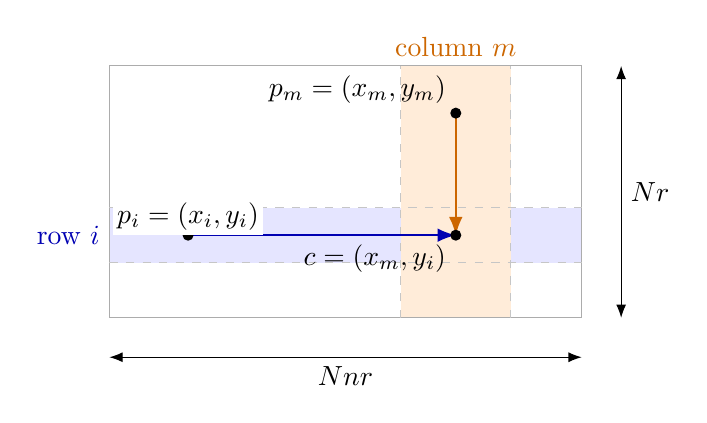
\begin{tikzpicture}[x=1cm,y=1cm,>=Latex]
 \fill[blue!10] (0,0.7) rectangle (6,1.4);
 \fill[orange!15] (3.7,0) rectangle (5.1,3.2);
 \draw[gray!65] (0,0) rectangle (6,3.2);
 \draw[gray!45,dashed] (0,0.7)--(6,0.7) (0,1.4)--(6,1.4);
 \draw[gray!45,dashed] (3.7,0)--(3.7,3.2) (5.1,0)--(5.1,3.2);
 \draw[blue!70!black,thick,->] (1.0,1.05)--(4.4,1.05);
 \draw[orange!80!black,thick,->] (4.4,2.6)--(4.4,1.05);
 \fill (1.0,1.05) circle (2pt) node[above,fill=white,inner sep=1.5pt] {$p_i=(x_i,y_i)$};
 \fill (4.4,2.6) circle (2pt) node[above left] {$p_m=(x_m,y_m)$};
 \fill (4.4,1.05) circle (2pt) node[below left] {$c=(x_m,y_i)$};
 \node[blue!70!black,left] at (0,1.05) {row $i$};
 \node[orange!80!black,above] at (4.4,3.2) {column $m$};
 \draw[<->] (0,-.5)--node[below] {$Nnr$}(6,-.5);
 \draw[<->] (6.5,0)--node[right] {$Nr$}(6.5,3.2);
\end{tikzpicture}
\caption{A schematic period block, for $i\ne m$. At $c$, both labels are allowed: $i$ by the row and $m$ by the column. Their normalized offsets are separated by at least $\sqrt2$. Transport along the arrows changes $h_i$ and $h_m$ by at most $\omega_n$ each, so $z_i=h_i(p_i)$ and $z_m=h_m(p_m)$ are separated by at least $\sqrt2-2\omega_n$. The block and strip proportions are schematic.}
\label{fig:crossing}
\end{figure}

For $i\ne m$, both added labels $re_{j,i}$ and $re_{j,m}$ are permitted at $(x_m,y_i)$: the first by row $i$, the second by column $m$. The corresponding source points have distance exactly $\sqrt2\,r$, so \eqref{eq:bilip} gives
\[
 \norm{h_i(x_m,y_i)-h_m(x_m,y_i)}\ge\sqrt2.
\]
Transporting along row $i$ and column $m$, as in Figure~\ref{fig:crossing}, yields
\[
 \norm{z_i-z_m}\ge\sqrt2-2\omega_n>1
\]
for all pairs when $n$ is sufficiently large. This is simultaneous because $N$ is fixed.

We have obtained $N$ points in the radius-$D$ ball of $\R^k$ with pairwise distances greater than one. Their open radius-$1/2$ balls are disjoint and contained in the radius-$(D+1/2)$ ball. Comparing Euclidean volumes gives
\[
 N(1/2)^k\le(D+1/2)^k,\qquad N\le(1+2D)^k,
\]
contrary to \eqref{eq:N}. No map satisfying \eqref{eq:bilip} exists. Together with Proposition~\ref{prop:doubling}, this proves Theorem~\ref{thm:main}.\qed

\section{A consequence for finite-\texorpdfstring{$p$}{p} function spaces}
\label{sec:lp}
A normalized Gaussian series gives isometric realizations of the same fixed metric space in real $L_p[0,1]$ for every finite $p\ge1$.

\begin{corollary}[Finite-$p$ function-space obstruction]\label{cor:lp}
For every real $1\le p<\infty$, the fixed metric space $S$ of Theorem~\ref{thm:main} is isometric to a subset $S_p$ of $L_p([0,1];\R)$, where $[0,1]$ carries Lebesgue measure. With its induced $L_p$ metric, $S_p$ has doubling constant at most $76800$ and admits no bi-Lipschitz embedding into any finite-dimensional real normed space at any finite distortion.
\end{corollary}
\begin{proof}
Fix $p$ and choose independent standard real Gaussian random variables $(g_i)_{i\ge1}$ on Lebesgue $[0,1]$. Put $c_p=(\mathbb E|g_1|^p)^{1/p}\in(0,\infty)$. For every finitely supported real sequence $a$, the sum $\sum_i a_i g_i$ is centered Gaussian with variance $\sum_i a_i^2$, and hence
\[
 \norm{\sum_i a_i g_i}_{L_p}=c_p\left(\sum_i a_i^2\right)^{1/2}.
\]
For $x\in\ell_2$, the same identity for tails makes the partial sums Cauchy in $L_p$. Completeness, including at $p=1$, therefore defines
\[
 J_p x=c_p^{-1}\lim_{m\to\infty}\sum_{i=1}^m x_i g_i
 \quad\text{in }L_p([0,1];\R).
\]
Passing to limits proves that $J_p$ is linear and that
$\norm{J_p x-J_p y}_{L_p}=\norm{x-y}_2$. Thus $S_p=J_p(S)$ is isometric to $S$, so its doubling constant is unchanged.

A zero-dimensional target cannot contain an injective copy of $S_p$. If $f:S_p\to Y$ were a bi-Lipschitz embedding into a real normed space of finite positive dimension $k$, choose a linear isomorphism $T:Y\to\R^k$. Equivalence of finite-dimensional norms makes $T$ bi-Lipschitz with finite distortion. The composition $T\circ f\circ J_p|_S$ would then contradict Theorem~\ref{thm:main}.
\end{proof}

Lafforgue and Naor proved the qualitative fixed-set obstruction with Euclidean targets for $p>2$ and, in the paragraph following their Theorem~1.1, recorded the corresponding question for $1<p\le2$ as open at that time, while noting stronger known results for $p=1$ \cite[Theorem 1.1 and the following paragraph]{LN}. Theorem~\ref{thm:main} treats $p=2$, and Corollary~\ref{cor:lp} answers that qualitative fixed-set question with finite-dimensional Euclidean targets when $1<p<2$. This transfer adds no new metric construction. Corollary~\ref{cor:lp} concerns function-space sources $L_p[0,1]$, not coordinate $\ell_p$ sources; the compact result below is a separate transfer to arbitrary infinite-dimensional Banach sources.

Finite-set dimension reduction in $L_p$, for $1<p<\infty$ and $p\ne2$,
allows the target dimension to depend on cardinality~\cite[Theorem~1.1]{OpenAI2026LpReduction},
unlike the fixed infinite-set obstruction of Corollary~\ref{cor:lp}.

\section{Compact obstructions in infinite-dimensional Banach spaces}
\label{sec:banach}
Finite witnesses to Theorem~\ref{thm:main} can be placed in any infinite-dimensional real Banach space by the classical Dvoretzky theorem. A geometrically shrinking union of these finite clusters, with its limit point adjoined, is compact and retains a uniform doubling bound.

\begin{corollary}[Compact Banach-space obstruction]\label{cor:banach}
There is a universal constant $\Lambda$ such that every infinite-dimensional real Banach space $B$ contains a compact subset $K_B$ whose doubling constant is at most $\Lambda$ and which admits no bi-Lipschitz embedding into any finite-dimensional real normed space at any finite distortion. The subset $K_B$ may depend on $B$, but is chosen independently of the target dimension and distortion.
\end{corollary}
\begin{proof}
Write $d_S$ for the induced Hilbert distance on $S$ and put $\lambda=76800$. We use closed balls below; the same estimates work for open balls.

\paragraph{Finite witnesses.}
For every $k\in\N$ and every finite $A\ge1$, there is a finite subset of $S$ admitting no embedding into $\R^k$ with distortion at most $A$. Indeed, suppose every finite subset admitted such an embedding, and fix $o\in S$. For each $x\in S$, let
\[
 Q_x=\{u\in\R^k:\norm u\le A d_S(o,x)\}.
\]
The product $\prod_{x\in S}Q_x$ is compact. In this product, each constraint
\[
 d_S(x,y)\le\norm{f(x)-f(y)}\le A d_S(x,y)
\]
defines a closed set. These closed sets have the finite-intersection property: finitely many constraints involve finitely many points, and an embedding of those points together with $o$, translated to send $o$ to zero and divided by its lower scale, satisfies the constraints and lies in the corresponding $Q_x$. Set all other coordinates to zero. Product compactness then supplies a map satisfying every constraint, contrary to Theorem~\ref{thm:main}.

Choose, for each $j\in\N$, a finite $X_j\subset S$ that admits no embedding into $\R^j$ with distortion at most $j$. Each $X_j$ has at least two points. These choices are made before any target for $K_B$ is considered.

\paragraph{Placement and cluster doubling.}
Fix an infinite-dimensional real Banach space $B$. The classical finite-dimensional Dvoretzky theorem \cite[Section~7]{Dvoretzky}, in the formulation recalled in \cite[Theorem~1.1]{COO}, gives a linear embedding $T_j$ of the finite Hilbert span of $X_j$ into $B$ with distortion strictly below two; the one-dimensional case is immediate. After rescaling $T_j$, we may use
\[
 d_S(x,y)\le\norm{T_jx-T_jy}_B\le2d_S(x,y)
 \qquad(x,y\in X_j).
\]
Only this qualitative finite-dimensional form of Dvoretzky is used.

Each $Y_j=T_j(X_j)$ has doubling constant at most $\lambda_0=\lambda^4$, uniformly in $j$ and $B$. To see this, the preimage $E$ of a ball in $Y_j$ of radius $R$ centered at $T_jx$ lies in the $S$-ball of radius $R$ centered at $x$. Four halvings cover that $S$-ball by at most $\lambda^4$ $S$-balls of radius $R/16$. For each one meeting $E$, choose $x_0\in E$ in it. Every other $x'\in E$ in the same ball satisfies
\[
 \norm{T_jx'-T_jx_0}_B
 \le2d_S(x',x_0)
 \le2\left(\frac R{16}+\frac R{16}\right)
 =\frac R4\le\frac R2.
\]
Thus the chosen points $T_jx_0$ give the required cover with centers in $Y_j$.

\paragraph{Compact assembly and its covering bound.}
Fix a unit vector $v\in B$, and put $a_j=2^{-j}$ and $\eta=1/100$. Since $Y_j$ is finite, a translation and positive rescaling place it as a cluster
\[
 C_j\subset B_B(a_jv,\eta a_j).
\]
This placement has distortion strictly below two as a map from $X_j$, and $C_j$ is still $\lambda_0$-doubling. Set
\[
 K_B=\{0\}\cup\bigcup_{j\ge1}C_j.
\]
For $z\in C_j$, one has $\norm z_B\le(1+\eta)a_j$. Every sequence in $K_B$ therefore has either a constant subsequence among $0$ and finitely many clusters, or a subsequence whose cluster indices tend to infinity and which converges to $0$. Hence $K_B$ is compact.

Fix $x\in K_B$ and $r>0$. Every cluster with $a_j\le r/4$, together with $0$, is covered by the single $K_B$-ball $B_{K_B}(0,r/2)$, since
\[
 \norm z_B\le(1+\eta)a_j\le\frac{101}{400}r<\frac r2
 \qquad(z\in C_j,\ a_j\le r/4).
\]
The center $0$ need not belong to the ball being covered. Let
\[
 I=\{j:C_j\cap B_{K_B}(x,r)\ne\varnothing,\ a_j>r/4\}.
\]
This is finite. If $i<j$, $p\in C_i$, and $q\in C_j$, then $a_j\le a_i/2$ and
\[
 \norm{p-q}_B
 \ge(a_i-a_j)-\eta(a_i+a_j)
 \ge\left(\frac12-\frac{3\eta}{2}\right)a_i
 =\frac{97}{200}a_i.
\]
If $|I|\ge2$, take its least index $i$ and any other $j\in I$. Points from the two intersections with $B_{K_B}(x,r)$ are at distance at most $2r$, so $a_i\le400r/97$. All scales indexed by $I$ then lie in $(r/4,(400/97)r]$. Their largest-to-smallest ratio is strictly less than $1600/97<32$, so there are at most five such dyadic scales. If $|I|=1$, its one scale can be arbitrarily large, but no bound on that scale is needed.

For each $j\in I$, choose $y_j\in C_j\cap B_{K_B}(x,r)$. The intersection is contained in the intrinsic $C_j$-ball $B_{C_j}(y_j,2r)$, which two applications of cluster doubling cover by at most $\lambda_0^2$ $C_j$-balls of radius $r/2$. The $K_B$-balls with these same centers and radii also cover the intersection. There are at most five clusters to cover, including the single-cluster case, so the tail ball and these covers use at most
\[
 1+5\lambda_0^2\le1+6\lambda^8
\]
balls, all centered in $K_B$. This proves a universal doubling bound; one may take $\Lambda=1+6\lambda^8$.

\paragraph{Obstruction for every finite-dimensional target.}
Suppose $K_B$ admitted a finite-distortion bi-Lipschitz embedding into a finite-dimensional real normed space. The zero-dimensional case is impossible because $K_B$ has more than one point. Otherwise, choose a linear isomorphism from the target onto $\R^k$. Equivalence of finite-dimensional norms makes this isomorphism bi-Lipschitz, so composition gives an embedding $f:K_B\to\R^k$ with some finite distortion $D$. Choose an integer $j\ge k$ with $j\ge2D$. Composing the distortion-below-two placement of $X_j$ onto $C_j$, the restriction of $f$, and the isometric inclusion $\R^k\hookrightarrow\R^j$ gives an embedding of $X_j$ into $\R^j$ with distortion strictly below $2D\le j$. This contradicts the choice of $X_j$.
\end{proof}

\begin{thebibliography}{99}
\bibitem{Assouad}
P. Assouad, \emph{Plongements lipschitziens dans $\R^n$},
Bulletin de la Soci\'et\'e Math\'ematique de France \textbf{111} (1983), 429--448.
\href{https://doi.org/10.24033/bsmf.1997}{doi:10.24033/bsmf.1997}.
\bibitem{BGN}
Y. Bartal, L.-A. Gottlieb, and O. Neiman, \emph{On the impossibility of dimension reduction for doubling subsets of $\ell_p$},
SIAM Journal on Discrete Mathematics \textbf{29} (2015), 1207--1222.
\href{https://doi.org/10.1137/140977655}{doi:10.1137/140977655}.
\bibitem{BSS}
F. P. Baudier, K. \'Swi\k{e}cicki, and A. Swift, \emph{No dimension reduction for doubling subsets of $\ell_q$ when $q>2$ revisited},
Journal of Mathematical Analysis and Applications \textbf{504} (2021), no.~2, 125407.
\href{https://doi.org/10.1016/j.jmaa.2021.125407}{doi:10.1016/j.jmaa.2021.125407}.
\bibitem{COO}
F. Catrina, S. Ostrovska, and M. I. Ostrovskii, \emph{Dvoretzky-type theorem for locally finite subsets of a Hilbert space},
Annales de l'Institut Fourier \textbf{75} (2025), no.~6, 2565--2607.
\href{https://doi.org/10.5802/aif.3672}{doi:10.5802/aif.3672}.
\bibitem{Cheeger}
J. Cheeger, \emph{Differentiability of Lipschitz functions on metric measure spaces},
Geometric and Functional Analysis \textbf{9} (1999), no.~3, 428--517.
\href{https://doi.org/10.1007/s000390050094}{doi:10.1007/s000390050094}.
\bibitem{Dvoretzky}
A. Dvoretzky, \emph{Some results on convex bodies and Banach spaces},
in Proceedings of the International Symposium on Linear Spaces
(Jerusalem, 1960), Jerusalem Academic Press, Jerusalem;
Pergamon Press, Oxford, 1961, 123--160.
\bibitem{GK}
L.-A. Gottlieb and R. Krauthgamer, \emph{A nonlinear approach to dimension reduction},
Discrete \& Computational Geometry \textbf{54} (2015), no.~2, 291--315.
\href{https://doi.org/10.1007/s00454-015-9707-9}{doi:10.1007/s00454-015-9707-9}.
\bibitem{GKL}
A. Gupta, R. Krauthgamer, and J. R. Lee, \emph{Bounded geometries, fractals, and low-distortion embeddings},
Proceedings of the 44th Annual IEEE Symposium on Foundations of Computer Science (2003), 534--543.
\href{https://doi.org/10.1109/SFCS.2003.1238226}{doi:10.1109/SFCS.2003.1238226}.
\bibitem{Heinonen}
J. Heinonen, \emph{Lectures on Lipschitz Analysis},
Report 100, Department of Mathematics and Statistics, University of Jyv\"askyl\"a, 2005.
\bibitem{Laakso}
T. J. Laakso, \emph{Ahlfors $Q$-regular spaces with arbitrary $Q>1$ admitting weak Poincar\'e inequality},
Geometric and Functional Analysis \textbf{10} (2000), no.~1, 111--123.
\href{https://doi.org/10.1007/s000390050003}{doi:10.1007/s000390050003}.
Erratum: ibid.\ \textbf{12} (2002), no.~3, 650.
\bibitem{LN}
V. Lafforgue and A. Naor, \emph{A doubling subset of $L_p$ for $p>2$ that is inherently infinite dimensional},
Geometriae Dedicata \textbf{172} (2014), 387--398.
\href{https://doi.org/10.1007/s10711-013-9924-4}{doi:10.1007/s10711-013-9924-4}.
\bibitem{LP}
U. Lang and C. Plaut, \emph{Bilipschitz embeddings of metric spaces into space forms},
Geometriae Dedicata \textbf{87} (2001), 285--307.
\href{https://doi.org/10.1023/A:1012093209450}{doi:10.1023/A:1012093209450}.
\bibitem{NN}
A. Naor and O. Neiman, \emph{Assouad's theorem with dimension independent of the snowflaking},
Revista Matem\'atica Iberoamericana \textbf{28} (2012), no.~4, 1123--1142.
\href{https://doi.org/10.4171/RMI/706}{doi:10.4171/RMI/706}.
\bibitem{OpenAI2026LpReduction}
OpenAI, \emph{Subpolynomial dimension reduction in $L_p$},
OpenAI Math Release preprint
\href{https://github.com/openai/math/blob/main/preprints/Subpolynomial-dimension-reduction-in-Lp-September-23-2026/paper.pdf}{OAI:Subpolynomial-dimension-reduction-in-Lp-September-23-2026},
2026.
\bibitem{Schioppa}
A. Schioppa, \emph{An example of a doubling ``inherently'' infinite-dimensional subset of $l_2$},
withdrawn preprint, 2017; withdrawal posted April 22, 2017.
\href{https://arxiv.org/abs/1703.10265}{arXiv:1703.10265}.
\bibitem{Tao}
T. Tao, \emph{245A, Notes 5: Differentiation theorems}, 16 October 2010,
\url{https://terrytao.wordpress.com/2010/10/16/245a-notes-5-differentiation-theorems/}.
\end{thebibliography}
\end{document}
